\documentclass[tikz,border=5pt,10pt]{standalone}
\usepackage{tikz}
\usetikzlibrary{calc}
\usepackage{pgf,xcolor}
\usepackage{eulervm}
\usepackage{booktabs,rotating,multirow,caption}
\usepackage{makecell}
\usetikzlibrary{automata}
\usetikzlibrary{arrows}
\usepackage{mathdots}
\usetikzlibrary{decorations.pathreplacing}
\usetikzlibrary{backgrounds}
\newcommand*\packet[1]{\tikz[baseline=(char.base)]{
            \node[thick,fill=white,shape=rectangle,draw,inner sep=2.5pt] (char) {#1};}}
\begin{document}
\begin{small}{\sffamily
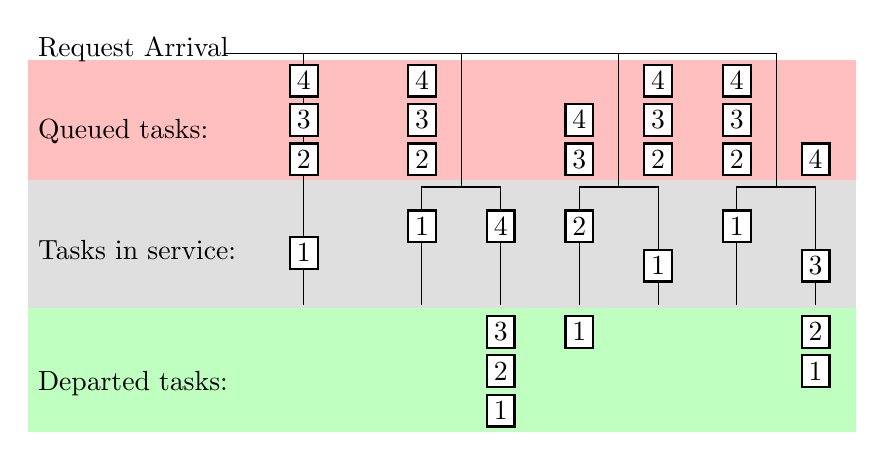
\begin{tikzpicture} %[line width=1.1pt]
\draw [fill=gray!25,gray!25] (-1.5,-1.41) rectangle (9,-3.05); 
\draw [fill=red!25,red!25] (-1.5,0.1) rectangle (9,-1.4); 
\draw [fill=green!25,green!25] (-1.5,-3.05) rectangle (9,-4.6); 
\node [right] at (-1.5,0.25) {Request Arrival};
%\node [left] at (1,0.25) {\packet{1}};
%\node [left] at (0.5,0.25) {\packet{2}};
%\node [left] at (0.,0.25) {\packet{3}};
%\node [left] at (-0.5,0.25) {\packet{4}};
\draw (1,0.2) -- (8,0.2);
%service
\draw (2,0.2) -- (2,-3);
\node [below] at (2,-2) {$\packet{1}$};
%queue
\node at (2,-1.15) {$\packet{2}$};
\node at (2,-0.65) {$\packet{3}$};
\node at (2,-0.15) {$\packet{4}$};
\draw (4,0.2) --(4,-1.5);
\draw (3.5,-3) --(3.5,-1.5)--(4.5,-1.5)--(4.5,-3);
%departed
\node  at (3.5,-2) {$\packet{1}$};
\node [below] at (4.5,-3) {$\packet{3}$};
\node [below] at (4.5,-3.5) {$\packet{2}$};
%service
\node [below] at (4.5,-4) {$\packet{1}$};
\node at (4.5,-2) {$\packet{4}$};
%queue
\node at (3.5,-1.15) {$\packet{2}$};
\node at (3.5,-0.65) {$\packet{3}$};
\node at (3.5,-0.15) {$\packet{4}$};
%
\draw (6,0.2) --(6,-1.5);
\draw (5.5,-3) --(5.5,-1.5)--(6.5,-1.5)--(6.5,-3);
%service
\node at (5.5,-2) {$\packet{2}$};
\node at (6.5,-2.5) {$\packet{1}$};
%queue
\node at (5.5,-1.15) {$\packet{3}$};
\node at (5.5,-0.65) {$\packet{4}$};
\node at (6.5,-1.15) {$\packet{2}$};
\node at (6.5,-0.65) {$\packet{3}$};
\node at (6.5,-0.15) {$\packet{4}$};
%departed
\node [below] at (5.5,-3) {$\packet{1}$};
%
\draw (8,0.2) --(8,-1.5);
\draw (7.5,-3) -- (7.5,-1.5)--(8.5,-1.5)--(8.5,-3);
%service
\node at (8.5,-2.5) {$\packet{3}$};
\node at (7.5,-2) {$\packet{1}$};
%queue
\node at (8.5,-1.15) {$\packet{4}$};
\node at (7.5,-1.15) {$\packet{2}$};
\node at (7.5,-0.65) {$\packet{3}$};
\node at (7.5,-0.15) {$\packet{4}$};
%departed
\node [below] at (8.5,-3) {$\packet{2}$};
\node [below] at (8.5,-3.5) {$\packet{1}$};
%
\node [right] at (-1.5,-.8) {Queued tasks:};
\node [right] at (-1.5,-4) {Departed tasks:};
\node [right] at (-1.5,-2.3) {Tasks in service:};
\end{tikzpicture}
}\end{small}
\end{document}